% -------------------------------------------------------------------------------- %

\begin{exercise}[Exercise 3.17]

What is the Bellman equation for action values, that is, for $q_\pi$?
It must give the action value $q_\pi(s, a)$ in terms of the action values, $q_\pi(s_0, a_0)$, of possible successors to the state-action pair $(s, a)$.
Hint:
the backup diagram to the right corresponds to this equation.
Show the sequence of equations analogous to \eqref{eq:3.8}, but for action values.

\end{exercise}

% -------------------------------------------------------------------------------- %

\begin{solution}

\phantom{}

\begin{center}
    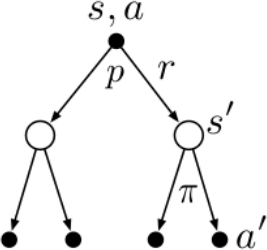
\includegraphics[width = 0.2 \textwidth]{1.17.png} \\
    $q_\pi$ backup diagram
\end{center}

\begin{align*}
    &
    q_\pi(s, a) \\
    & \doteq
    \E_\pi [G_t \mid S_t = s, A_t = a] \\
    & =
    \E_\pi [R_{t+1} + \gamma G_{t+1} \mid S_t = s, A_t = a] \\
    & =
    \sum_{s^\prime, r}
        p(s^\prime, r \mid s, a)
        \E_\pi[R_{t+1} + \gamma G_{t+1} \mid S_t = s, A_t = a, S_{t+1} = s^\prime, R_{t+1} = r] \\
    & =
    \sum_{s^\prime, r}
        p(s^\prime, r \mid s, a)
        \sum_{a^\prime}
            \pi(a^\prime \mid s^\prime) \\ & \quad
            \E_\pi[R_{t+1} + \gamma G_{t+1} \mid S_t = s, A_t = a, S_{t+1} = s^\prime, R_{t+1} = r, A_{t+1} = a^\prime] \\
    & =
    \sum_{s^\prime, r}
        p(s^\prime, r \mid s, a)
        \sum_{a^\prime}
            \pi(a^\prime \mid s^\prime) \\ & \quad
            \sum_{r^\prime}
                r^\prime
                \Pr \Bbraces{R_{t+1} + \gamma G_{t+1} = r^\prime \mid S_t = s, A_t = a, S_{t+1} = s^\prime, R_{t+1} = r, A_{t+1} = a^\prime} \\
    & =
    \sum_{s^\prime, r}
        p(s^\prime, r \mid s, a)
        \sum_{a^\prime}
            \pi(a^\prime \mid s^\prime) \\ & \quad
            \sum_{r^\primeprime}
                (r + \gamma r^\primeprime)
                \Pr \Bbraces{G_{t+1} = r^\primeprime \mid S_{t+1} = s^\prime, A_{t+1} = a^\prime} \\
    & =
    \sum_{s^\prime, r}
        p(s^\prime, r \mid s, a)
        \sum_{a^\prime}
            \pi(a^\prime \mid s^\prime) \\ & \quad
            \pbraces
            {
                r
                \sum_{r^\primeprime}
                    \Pr \Bbraces{G_{t+1} = r^\primeprime \mid S_{t+1} = s^\prime, A_{t+1} = a^\prime}
                +
                \gamma 
                \sum_{r^\primeprime}
                    r^\primeprime
                    \Pr \Bbraces{G_{t+1} = r^\primeprime \mid S_{t+1} = s^\prime, A_{t+1} = a^\prime}
            } \\
    & =
    \sum_{s^\prime, r}
        p(s^\prime, r \mid s, a)
        \sum_{a^\prime}
            \pi(a^\prime \mid s^\prime) \\ & \quad
            \pbraces
            {
                r
                +
                \gamma 
                \E_\pi[G_{t+1} \mid S_{t+1} = s^\prime, A_{t+1} = a^\prime]
            } \\
    & =
    \sum_{s^\prime, r}
        p(s^\prime, r \mid s, a)
        \sum_{a^\prime}
            \pi(a^\prime \mid s^\prime) \\ & \quad
            \pbraces
            {
                r
                +
                \gamma
                q_\pi(s^\prime, a^\prime)
            }
\end{align*}

\end{solution}

% -------------------------------------------------------------------------------- %
